\chapter{O que se desaprende}\label{cap:desaprende}

A média de tudo é o estimador mais antigo que existe, e é o único que ninguém precisa escolher: ele
cai de graça de quem não quer decidir. No dia $t$ ele dá o mesmo peso a todos os $t$ dias que já viu,
de modo que a memória dele é a própria idade. Este capítulo mede o que isso cobra --- e o que custa
escolher outra coisa.

\section{A memória que envelhece}

O capítulo da memória mediu a taxa com que o passado cede lugar ao presente, e escolheu-a por
medição: vinte e um dias, com o horizonte que a tabela de lá declara. Mas ninguém é obrigado a
escolher taxa nenhuma, e o caminho sem escolha tem nome: a média acumulada. Ela é a primeira coisa
que qualquer um escreve, e é o que fica quando ninguém decide.

A proposição da meia-vida cobre esse caso sem que ninguém o tenha pedido. Com a taxa que a idade
impõe --- um sobre $t$ no dia $t$ ---, os dias para o erro cruzar a tolerância crescem com a idade:
aos vinte e um dias de uso a conta pede \numAprenderDiasVinteEUm{} dias, aos cinquenta pede
\numAprenderDiasCinquenta{}, aos duzentos e cinquenta pede \numAprenderDiasDuzentosECinquenta{} e aos
mil pede \numAprenderDiasMil. Não é coincidência: essas são as quatro linhas que o capítulo da
memória já imprime, e a conta da idade as reproduz com erro de \numAprenderErroMaximoPct{}\% --- a
previsão e o impresso são a mesma conta, e agora está dito.

O que isso quer dizer na série do livro é o tamanho do problema. Aos \numAprenderDiasSerie{} dias de
série, a idade do fim pede \numAprenderDiasSerieConta{} dias para aprender o nível novo:
\numAprenderRazaoSerie{} vezes a série inteira. \textbf{Quem nunca esquece não alcança o próprio
passado} --- e o que ele faz não é guardar, é atrasar.

\begin{figure}[htbp]
  \centering
  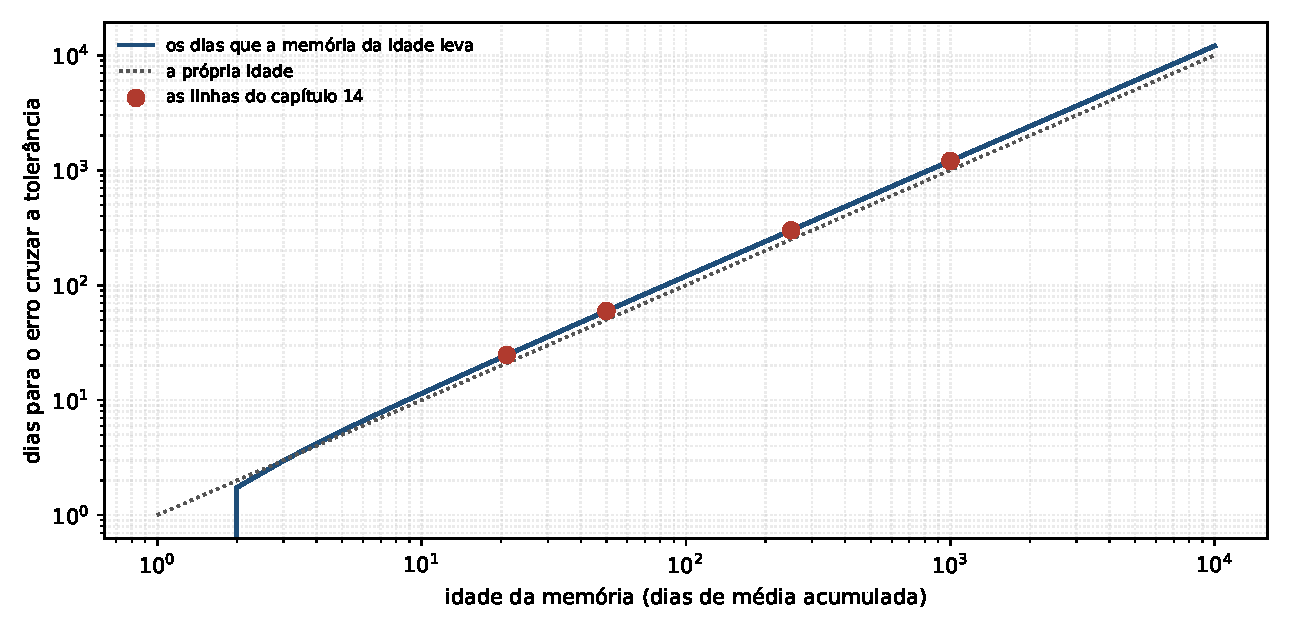
\includegraphics[width=\linewidth]{figuras/E26_aprender_1.pdf}
  \caption{Os dias que a memória da idade leva para cruzar a tolerância, contra a idade dela. Os
    dois eixos são logarítmicos; a linha pontilhada é a própria idade, e os pontos são as quatro
    linhas que o capítulo da memória já publicava. A curva e a reta são paralelas, e é isso que faz
    do caso um caso sem conserto.}
  \label{fig:idade}
\end{figure}

A distância entre a curva e a reta não cresce com a idade: ela fica em torno de vinte por cento em
toda a escala --- a razão vale \numAprenderRazaoVinteEUm{} aos vinte e um dias e
\numAprenderRazaoMil{} aos mil. Quem nunca esquece não fica cada vez mais para trás: fica sempre a
mesma fração atrás, e é por isso que esperar não resolve.

\section{O que custa escolher}

O conserto é o do capítulo da memória --- escolher a taxa em vez de herdar a idade ---, e o preço
dele se mede. Quatro estimadores, o mesmo degrau no dia \numConsertoQuando{}, o mesmo horizonte de
\numConsertoHorizonte{} dias e o mesmo mundo de \numConsertoDias{} dias: a média acumulada, a
exponencial de vinte e um dias, a acumulada que reinicia a cada \numConsertoJanela{} dias e a janela
de \numConsertoJanela{} dias.

\begin{table}[htbp]
  \centering
  \small
  \begin{tabular}{lr}
    \hline
    estimador & erro depois do degrau \\
    \hline
    a janela de \numConsertoJanela{} dias & \numConsertoErroJanela \\
    a exponencial de vinte e um dias & \numConsertoErroExponencial \\
    a média acumulada & \numConsertoErroAcumulada \\
    a acumulada que reinicia & \numConsertoErroReinicia \\
    \hline
  \end{tabular}
  \caption{O erro de cada estimador no mesmo horizonte, em \numConsertoMundos{} mundos. O degrau é o
    do capítulo da memória, e a tolerância daquele capítulo é de \numEsquecimentoTolerancia{} do
    nível novo.}
  \label{tab:conserto}
\end{table}

A ordem é a lição. \textbf{Escolher a memória corta o erro para menos da metade}: a pior das quatro
erra \numConsertoRazaoPiorMelhor{} vezes o que a melhor erra. E o conserto ingênuo não é conserto: a
acumulada que reinicia a cada janela erra \numConsertoErroReinicia, mais do que a que nunca esquece
--- uma média recém-nascida é tão cega quanto uma média velha é surda, e reiniciar só troca uma
cegueira pela outra.

\begin{figure}[htbp]
  \centering
  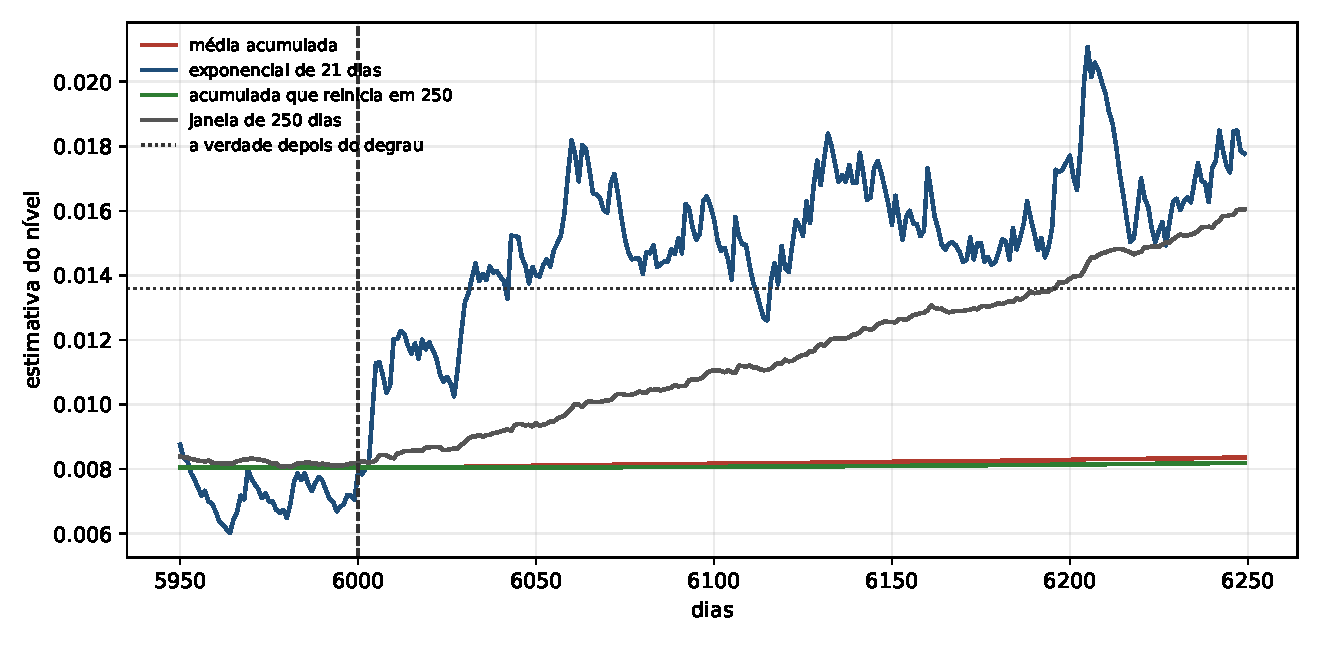
\includegraphics[width=\linewidth]{figuras/E27_conserto_1.pdf}
  \caption{Os quatro estimadores em torno do dia do degrau, contra a verdade. Depois dele a
    exponencial de vinte e um dias reage e oscila em volta da linha; a janela sobe em rampa, porque
    vai sendo preenchida por dias novos; e a média acumulada e a que reinicia ficam paradas --- elas
    carregam tanto passado que o degrau quase não as move dentro do horizonte da decisão.}
  \label{fig:conserto}
\end{figure}

\section{Quantos dias a memória devolve}

A tabela anterior mediu o preço de escolher; falta o porquê, e ele tem número. Cada memória é um
% aterramento: capacidade
estado que anda com a série --- e a pergunta da capacidade é quantos dias individuais do passado
% aterramento: readout
esse estado devolve, por leitura linear, medida fora da amostra: o readout é ajustado numa metade
dos dias e a capacidade é a correlação ao quadrado entre o que ele devolve e o dia, na outra metade
--- porque capacidade medida dentro da amostra é ajuste, não memória. A soma sobre os atrasos tem
teto: não passa do posto da matriz de controlabilidade, que não passa da dimensão do estado --- o
% aterramento: posto-do-estado
posto do estado --- a
dinâmica distribui a capacidade, não a cria \cite{dambre2012information}.

Os quatro sistemas do capítulo, agora como estados. A resposta seca:

\begin{itemize}
\item a acumulada devolve \numCapacidadeAcumuladaTotal{} --- zero dias: a direção que ela guarda é a
média, e média nenhuma é dia;
\item a exponencial da meia-vida de vinte e um dias devolve \numCapacidadeExponencialTotal{} ---
menos de uma direção inteira: um número só carrega no máximo um passado, e nem inteiro;
\item a janela devolve \numCapacidadeJanelaTotal{}: os duzentos e cinquenta, inteiros, e nada além
--- mais os empréstimos do acaso nos mil e duzentos e cinquenta atrasos além da parede, que somam
menos que um dia;
\item o reservatório --- estado de cem números, matriz esparsa com raio espectral abaixo de um, a
condição de estado de eco \cite{jaeger2001echo}, da família que computa em tempo real sem estados
estáveis \cite{maass2002real} e cuja aproximação tem teorema \cite{hart2020embedding} --- devolve
\numCapacidadeReservatorioTotal{} [\numCapacidadeReservatorioTotalMin;
\numCapacidadeReservatorioTotalMax] de cem.
\end{itemize}

\begin{figure}[htbp]
  \centering
  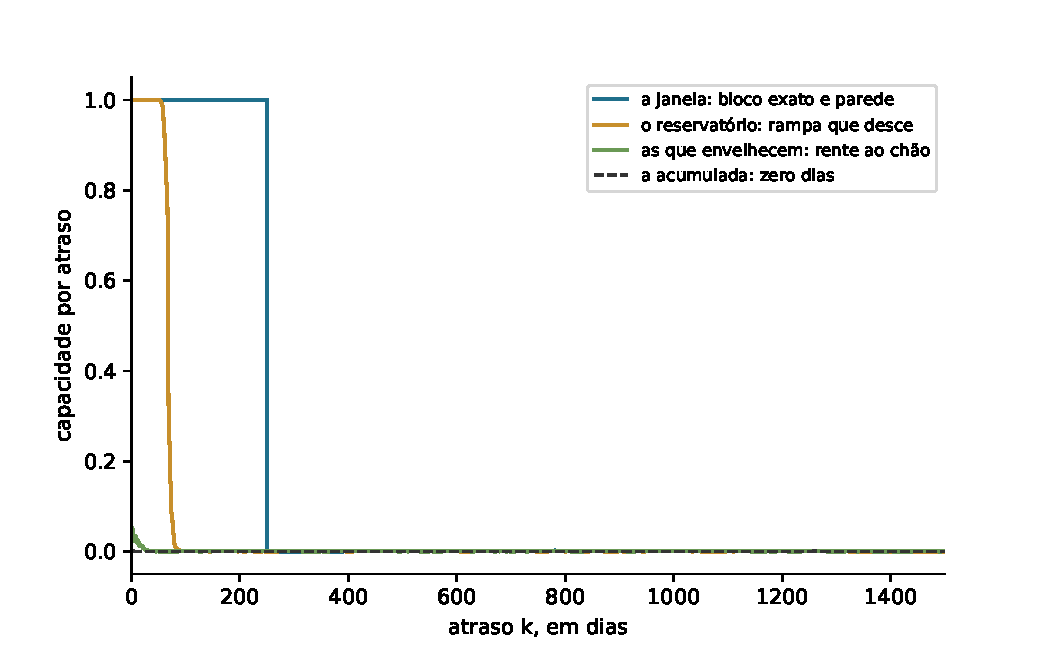
\includegraphics[width=\linewidth]{figuras/E41_capacidade_1.pdf}
  \caption{O perfil da capacidade por atraso. A janela é bloco exato com parede; o reservatório é
    rampa que desce --- no atraso \numCapacidadeReservatorioLagMetade{} a capacidade por atraso cai à
    metade do primeiro atraso; e as duas que envelhecem ficam rente ao chão desde o primeiro dia.}
  \label{fig:capacidade_perfil}
\end{figure}

E aqui está o porquê da tabela. A acumulada perde porque não tem onde pôr os dias: capacidade zero
para dias individuais é cegueira de fabricação, não erro de cálculo. A janela ganha dentro dos seus
duzentos e cinquenta dias porque guarda os dias, um por número --- e o preço dela é a parede. O
reservatório é a terceira via: espalha os seus cem números por um passado profundo, não devolve dia
nenhum inteiro e não tem parede --- mas não enche o posto: com os dias que o mercado deu, dois terços
da dimensão. O teto do teorema é o teto; o dado é que não chega.

\begin{figure}[htbp]
  \centering
  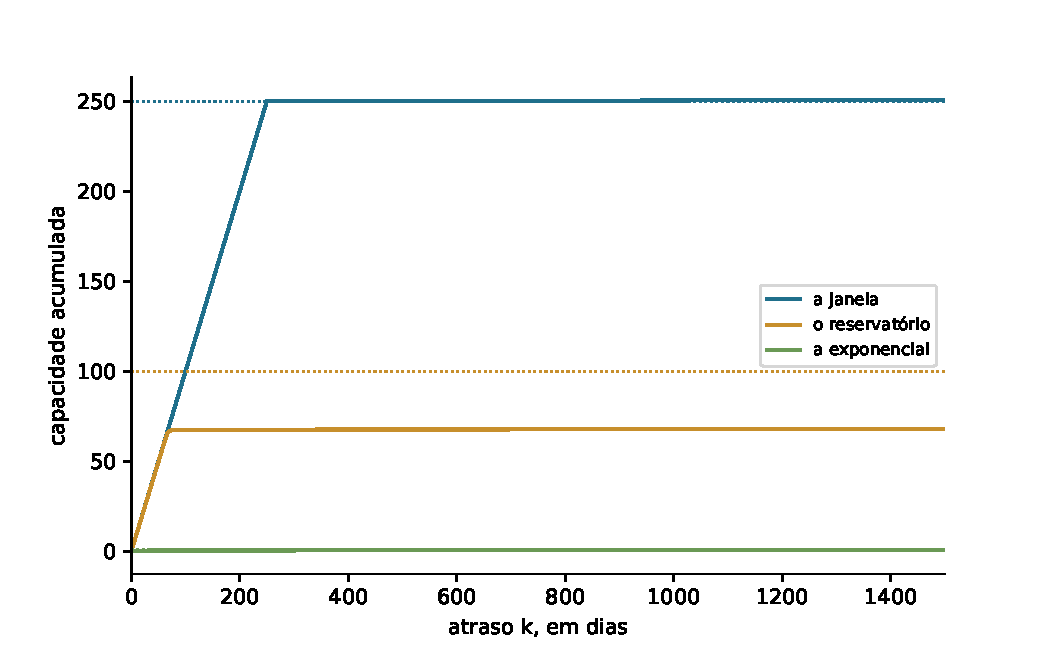
\includegraphics[width=\linewidth]{figuras/E41_capacidade_2.pdf}
  \caption{A capacidade acumulada contra o atraso, com o tamanho de cada estado pontilhado. A janela
    satura na parede e para; o reservatório sobe devagar e satura antes do seu tamanho; as que
    envelhecem nem saem do chão.}
  \label{fig:capacidade_acumulada}
\end{figure}

O que o capítulo fecha, então, é a conta inteira: escolher a memória é escolher onde a capacidade
mora --- bloco exato com parede, rampa profunda sem garantia de dia, ou uma direção que não é dia
nenhum. O teto do que se aprende, medido no capítulo seguinte, tem o gêmeo aqui: o teto do que se
lembra é o tamanho do estado, e nenhuma dinâmica compra memória de graça.

\section{A promessa sobre dias que não vieram}

A seção anterior construiu o instrumento e mediu quanto ele lembra. Falta a pergunta seguinte,
sobre o mesmo instrumento: quanto ele pode \emph{prometer} sobre os dias que não viu. A resposta
tem dois lados --- uma contagem e um preço --- e os dois se medem.

% aterramento: funcao-de-crescimento
O primeiro lado é de contagem \cite{vapnik1971uniform}. O readout encaixa uma dicotomia sorteada de \emph{n} dias com erro
zero quando os dias cabem no que o estado distingue, e não encaixa quando não cabem. Medida a
fração de dicotomias encaixadas em \numPromessaGradeSeparacoes{} tamanhos, dos
\numPromessaDimensaoExponencial{} estado da memória exponencial ao de
\numPromessaDimensaoReservatorio{} do reservatório, o resultado tem forma de degrau: a memória
exponencial desaba em \numPromessaDesabaExponencial{} dias, o reservatório em
\numPromessaDesabaReservatorio, e a janela de \numPromessaDimensaoJanela{} dias ainda encaixa tudo
no maior tamanho medido. \textbf{O teto da promessa vem da contagem} --- a \textbf{função de crescimento} da classe ---, e não do número de
parâmetros: e a contagem do reservatório é menor do que a dimensão dele --- o sorteio da matriz
esparsa não põe todos os estados a trabalhar.

\begin{figure}[htbp]
  \centering
  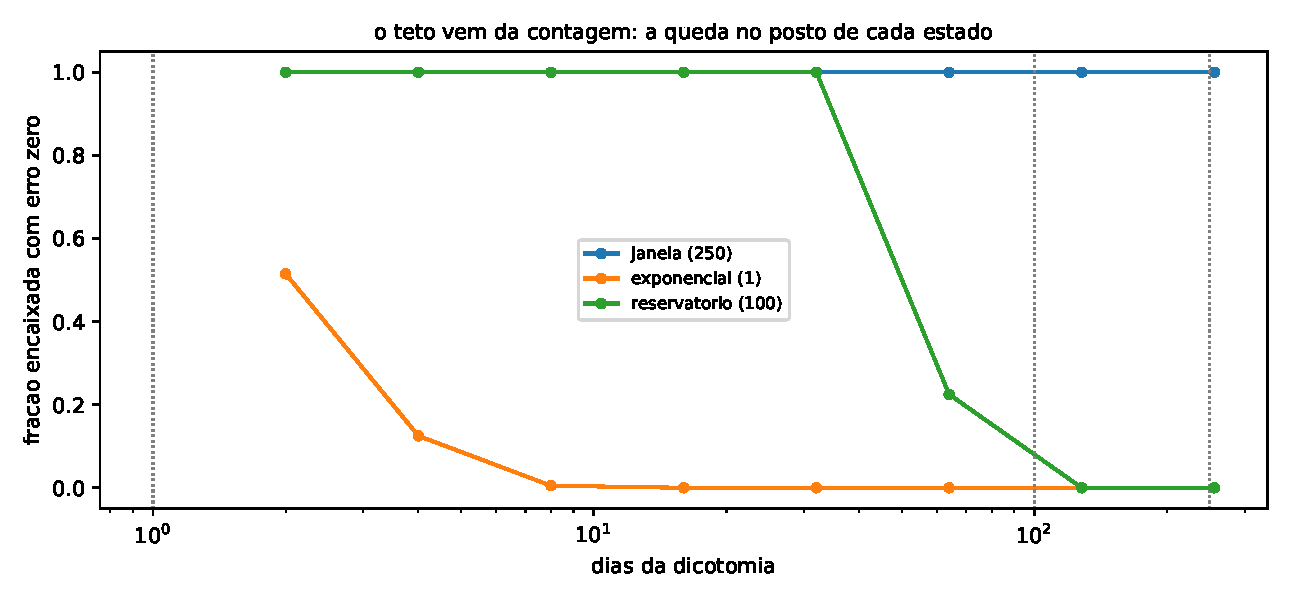
\includegraphics[width=\linewidth]{figuras/E53_promessa_1.pdf}
  \caption{A fração de dicotomias encaixadas com erro zero contra o número de dias, nos três
    estados, com a linha pontilhada da dimensão de cada um. As curvas valem um e desabam no degrau
    de cada estado. A do reservatório desaba antes da própria dimensão, e a da memória
    exponencial desaba no primeiro tamanho em que a fração cai abaixo de meio.}
  \label{fig:contagem}
\end{figure}

% aterramento: rademacher
O segundo lado é de geometria. A \textbf{complexidade de Rademacher} da classe de leituras
lineares se mede por sorteio de rótulos \cite{kakade2008complexity}: para cada sorteio de sinais, o quanto a classe consegue
alinhar ruído puro. Contra os dias, ela decai: em \numPromessaRademacherDias{} dias vale
\numPromessaRademacherMedia, contra a conta fechada de \numPromessaRademacherRazao{} --- o mesmo
número, na mesma ordem, e as duas curvas são a mesma reta no desenho. O que a cota cobra é o raio
dos dados vezes a norma dos pesos, e não o número de pesos.

\begin{figure}[htbp]
  \centering
  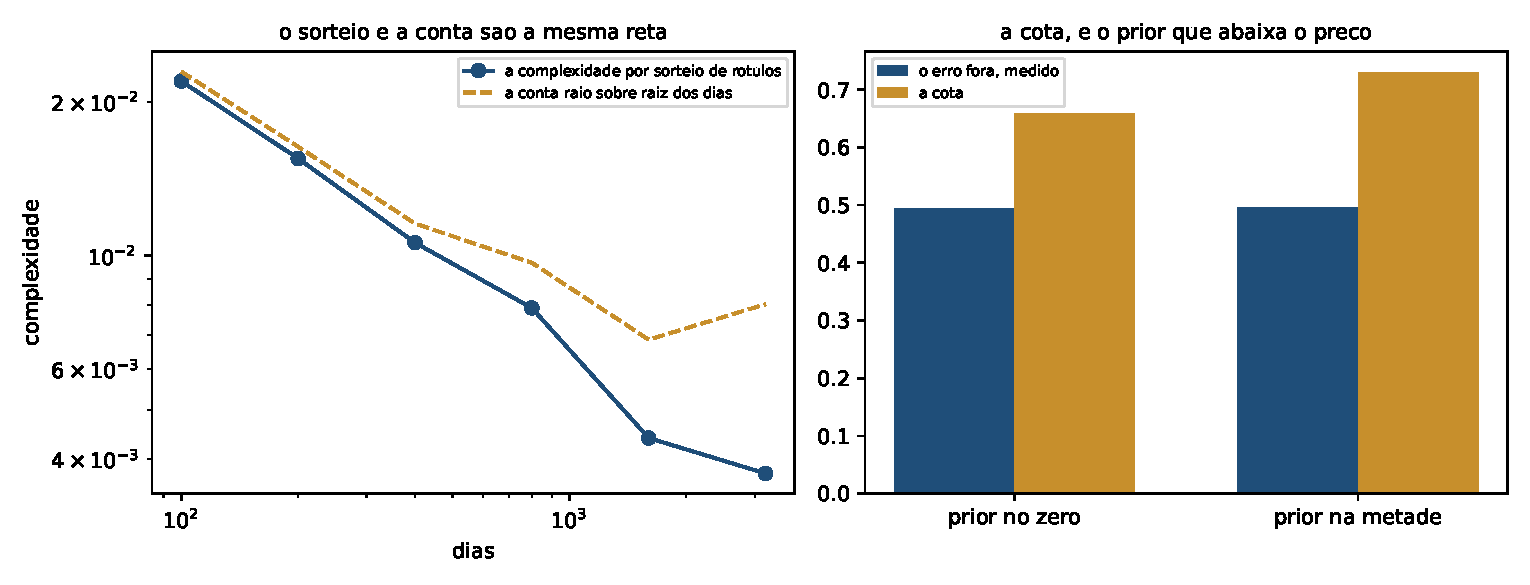
\includegraphics[width=\linewidth]{figuras/E53_promessa_2.pdf}
  \caption{À esquerda, a complexidade por sorteio de rótulos contra os dias, com a conta fechada
    do raio sobre a raiz dos dias: as duas curvas descem juntas. À direita, o erro fora medido e a
    cota, nos dois braços --- a barra da cota fica acima da barra do erro.}
  \label{fig:rademacher}
\end{figure}

% aterramento: divergencia-em-bits
% aterramento: prior
O preço tem nome e unidade. Com o readout perturbado, o erro fora é de \numPromessaForaZero{} com o
prior no zero e de \numPromessaForaMetade{} com o prior que já viu a metade da amostra, e as duas
cotas ficam acima \cite{seeger2002bayesian}: \numPromessaCotaZero{} e \numPromessaCotaMetade, com folgas de
\numPromessaFolgaZero{} e \numPromessaFolgaMetade. O preço é a \textbf{divergência em bits} entre a
hipótese escolhida e o \textbf{prior} --- \numPromessaKlZeroBits{} bits no braço do zero.

E aqui a medição desmente o que a fonte sugere. O prior dependente da instância não abaixou o
preço: ele o subiu, de \numPromessaKlZeroBits{} para \numPromessaKlMetadeBits{} bits ---
\numPromessaPriorAbaixaBits{} bits a mais. A razão é a estabilidade que a fonte exige e que este
instrumento não tem: os readouts das duas metades ficam longe um do outro, e um prior que aponta
para o lugar errado cobra mais do que o prior que não aponta para lugar nenhum. A cota continua
valendo nos dois braços --- ela fica \emph{acima} do erro medido nos dois ---, e o que ela carrega
a mais é isso: o preço da instabilidade \cite{rivasplata2018bayes}.

% aterramento: unidade-dormente
Falta o teto medido depois do uso, que é a pergunta do título deste capítulo. Com o número de
estados fixo, a sonda fresca mede a capacidade em \numPromessaBlocos{} blocos: o reservatório
linear fica plano, de \numPromessaTetoLinearInicio{} a \numPromessaTetoLinearFim, e é o controle
que isola a causa. O que satura perde \numPromessaSaturadoPerdaPct\% do teto no mesmo percurso ---
pouco, e menos do que o desenho esperava. E a realocação não mudou nada: a fração de
\textbf{unidades dormentes} ficou em \numPromessaDormentesMediaPct\% e a perda do braço realocado
é a mesma do saturado, \numPromessaRealocadoPerdaPct\%. \textbf{A dormente não mora aqui} --- a
saturação não engatou neste instrumento, e o contraste que a fonte descreve \cite{dohare2024loss} fica declarado sem
medição.

\begin{figure}[htbp]
  \centering
  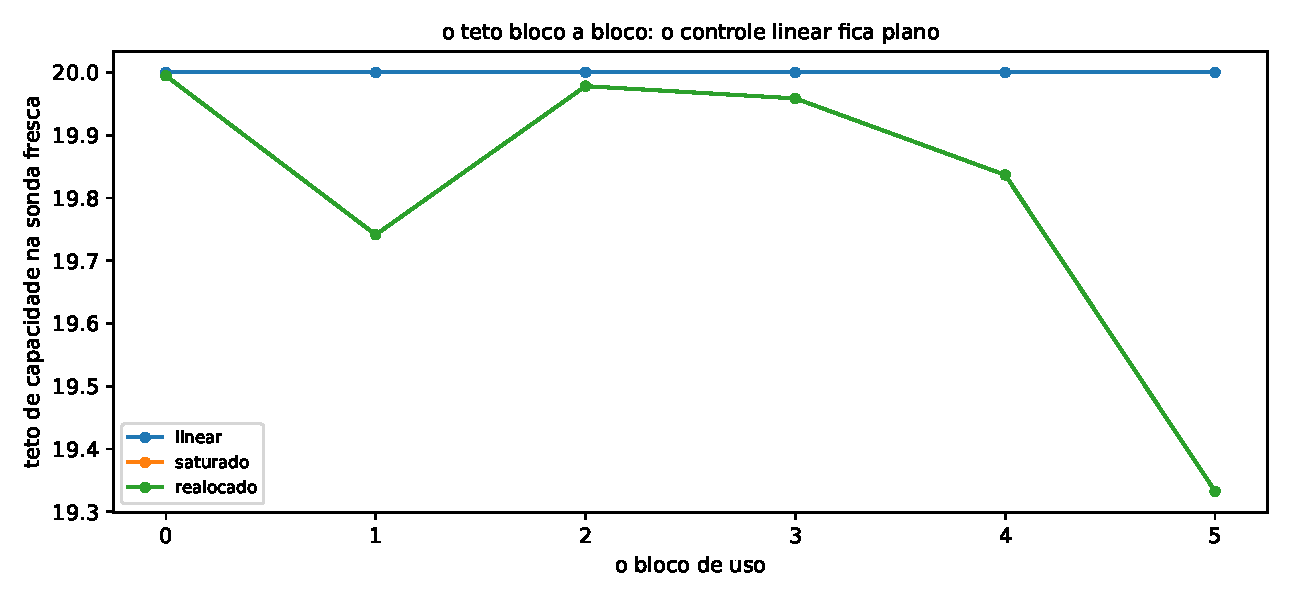
\includegraphics[width=\linewidth]{figuras/E53_promessa_3.pdf}
  \caption{O teto de capacidade medido numa sonda fresca depois de cada bloco de uso, nas três
    curvas. A do reservatório linear fica plana; a do saturado e a do realocado descem juntas ---
    a realocação não mudou nada, porque não havia dormente para realocar.}
  \label{fig:uso}
\end{figure}

O que fica é a promessa com as duas metades declaradas: o teto vem da contagem --- e a contagem
efetiva é menor do que a dimensão ---, e o preço vem em bits, cobrado do erro dentro para prometer
o de fora. O que o capítulo seguinte acrescenta é o pedaço: a cota foi medida num trecho da série
e num mundo que não mudou entre as metades.

\section{O que fica}

Fica a resposta, e ela é estreita: o estimador mais barato de escrever é o mais caro de usar. A
memória não é um resíduo da idade do sistema --- é uma escolha, e escolhê-la tem preço declarado,
medido no mesmo horizonte em que a decisão acontece.

O que sobra é o fracasso seguinte, e ele é do tamanho da escolha que se acabou de fazer. A taxa do
capítulo da memória foi medida num mundo que ou não muda ou dobra de uma vez, e a desta seção, no
mesmo mundo. \textbf{Escolher a memória exige saber quanto tempo o mundo fica parado} --- e esse
tempo não é um dado da série: é uma borda que quem decide declara. É o que o enquadramento vai
medir: onde a série começa e termina, de quando é o dado que chega, e quanto passado ainda conta.
